\documentclass{kougai}
\usepackage{graphicx}

\papertitle{ここに梗概のタイトル}
%\papertitle{梗概のタイトル \\  長くて2行になる場合はこちら}
\studentno{ここに学籍番号}
\studentname{ここに姓　ここに名}
\advisor{ここに姓　ここに名　教授}

\begin{document}
\makekougaititle

\section{はじめに}
研究の背景と目的を書きます．何が問題で，この研究で何をするのかを簡潔にまとめます．
研究の背景と目的を書きます．何が問題で，この研究で何をするのかを簡潔にまとめます．

\section{関連研究}
先行研究とその課題を書きます．文献を引用するときは\cite{yamada2025}のように書きます．
先行研究とその課題を書きます．先行研究とその課題を書きます．

\section{提案方式}
提案する手法を書きます．提案する手法を書きます．提案する手法を書きます．
提案する手法を書きます．提案する手法を書きます．

\section{実験概要と結果}
実験の環境と条件，結果を書きます．図は図\ref{fig:sample}のように参照します．
実験の環境と条件，結果を書きます．表は表\ref{tab:sample}のように参照します．

\begin{table}[t]
    \caption{表の例}
    \label{tab:sample}
    \centering
    \begin{tabular}{cccc}
    \hline
           & A    & B    & C    \\ \hline
    条件1  & 1.00 & 2.00 & 3.00 \\
    条件2  & 1.50 & 2.50 & 3.50 \\ \hline
    \end{tabular}
\end{table}

\begin{figure}[t]
    \centering
    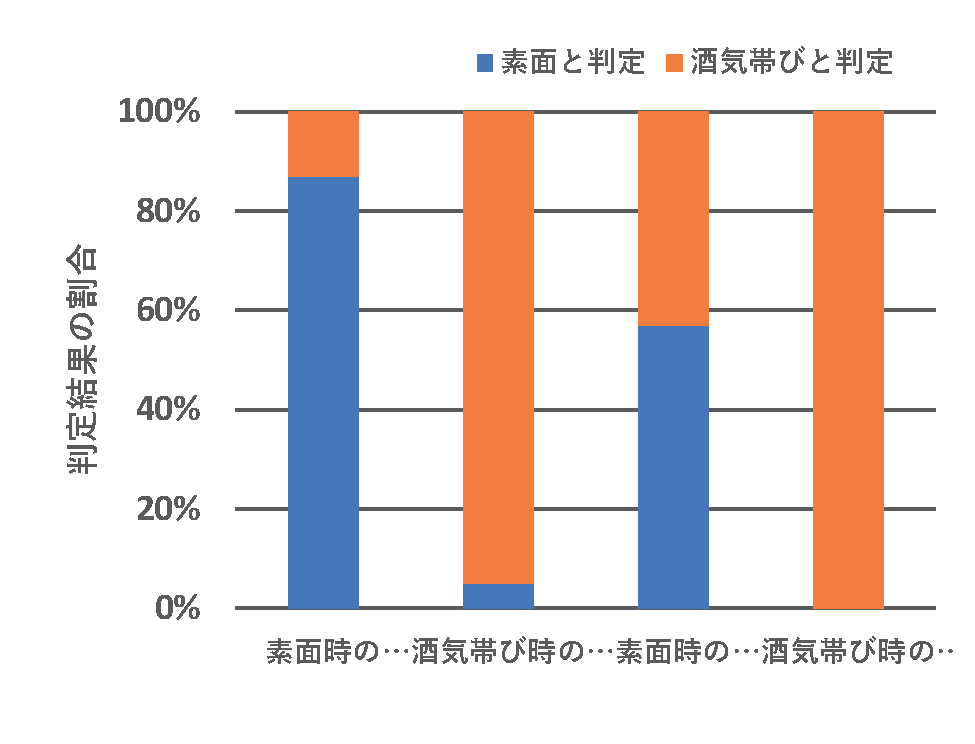
\includegraphics[width=6cm]{Figures/sample.eps}
    \caption{図の例}
    \label{fig:sample}
\end{figure}

\section{まとめ}
研究のまとめと今後の課題を書きます．研究のまとめと今後の課題を書きます．

\bibliographystyle{../junsrt}
\bibliography{../references}

\end{document}
